%! program = pdflatex

\documentclass[12pt]{article}
\usepackage{amsmath}
\usepackage{natbib}
\usepackage{graphicx}
\usepackage{amssymb}
\usepackage{epstopdf}
\usepackage{float} % to keep the figures in place
\usepackage{placeins}

\usepackage{caption}
\usepackage{subcaption}
\usepackage{color}
\usepackage{undertilde}
\usepackage{enumitem}
\newcommand{\cred}{ \color{red}}
\newcommand{\cgreen}{\color{green}}
\newcommand{\cblue}{\color{blue}}
\newcommand{\cmag}{\color{magenta}}
\newcommand{\bn}{\begin{enumerate}}
\newcommand{\en}{\end{enumerate}}
\newcommand{\bi}{\begin{itemize}}
\newcommand{\ei}{\end{itemize}}
\newcommand{\be}{\begin{eqnarray}}
\newcommand{\ee}{\end{eqnarray}}
\newcommand{\by}{\begin{eqnarray*}}
\newcommand{\ey}{\end{eqnarray*}}
\renewcommand{\labelenumi}{(\alph{enumi}) }

\usepackage[margin=2.2cm, includehead]{geometry}% see geometry.pdf on how to lay out the page. There's lots.
\geometry{letterpaper} % or letter or a5paper or ... etc
% \geometry{landscape} % rotated page geometry
%\bibpunct{(}{)}{;}{a}{,}{,}
%\setlength{\textwidth}{16cm}
%\setlength{\textheight}{21cm}
\def\nonumber{\global\@eqnswfalse}
\newcounter{parnum}
\newcommand{\N}{%
  \noindent\refstepcounter{parnum}%
   \makebox[\parindent][l]{\textbf{[\arabic{parnum}]}}\quad  }
% Use a generous paragraph indent so numbers can be fit inside the
% indentation space.
\setlength{\parindent}{1.5em}

% See the ``Article customise'' template for come common customisations

\date{}
%\date{} % delete this line to display the current date

%%% BEGIN DOCUMENT
\usepackage{Sweave}
\begin{document}
\Sconcordance{concordance:aua257HW4.tex:aua257HW4.Rnw:%
1 51 1 1 0 49 1 1 85 1 3 9 1 1 4 12 1 1 45 4 1 1 5 1 2 5 1 1 12 6 1}

%\large
%\maketitle
\newtheorem{thm}{Theorem}[section]
\newtheorem{cor}[thm]{Corollary}
\newtheorem{lem}[thm]{Lemma}
\newtheorem{prop}[thm]{Proposition}
\newtheorem{defn}[thm]{Definition}
\newtheorem{exam}[thm]{Example}
\newtheorem{qstn}[thm]{Question}

%%%
\newpage
\begin{center}
{\bf Homework 4 - STAT 540}\\
Amal Agarwal
\end{center}
%==========================
\section*{Answer 1}
Given that $A_1, A_2, ..., A_m \sim \text{Exponential}(\theta)$. Assume we observe $Y_1, Y_2, ..., Y_m$, where $Y_i:=\text{min}(A_i,\tau)$ where $\tau=100$ days. The observed log-likelihood function which is needed to be maximized is w.r.t. $\theta$ is \[l_{\text{obs}}(\theta)=\sum\limits_{i: Y_i<\tau}\left(-\text{log}(\theta)-\dfrac{Y_i}{\theta}\right)+\sum\limits_{i: Y_i=\tau}\left(\dfrac{-Y_i}{\tau}\right)\] 
The complete log-likelihood function can be written as
\[l_{\text{comp}}(\theta)=\sum\limits_{i=1}^m\left(-\text{log}(\theta)-\dfrac{A_i}{\theta}\right)\]

The pseudocode for the algorithm is given as follows:
\begin{enumerate}[label=(\alph*)]
\item Start off with some initial guess for $\theta^{(1)}$.
\item At the $k^{\text{th}}$ iterate of EM algorithm, the E-step involves writing down surrogate function which is the expectation of complete log likelihood function as defined above given the observed data $\utilde{Y}$ and $\theta^{(k)}$. This can be evaluated as follows:

\begin{equation}
\begin{aligned}
E_{\theta^{(k)}}(l_{\text{comp}}(\theta)|\utilde{Y})&=\sum\limits_{i: Y_i<\tau}\left(-\text{log}(\theta)-\dfrac{Y_i}{\theta}\right)+\sum\limits_{i: Y_i=\tau}\left(-\text{log}(\theta)-\dfrac{E_{\theta^{(k)}}(X_i|\utilde{Y})}{\theta}\right)\\&=-m\text{log}(\theta)-\dfrac{\sum\limits_{i: Y_i<\tau}Y_i}{\theta}-\dfrac{(\tau+\theta^{(k)})(m-u)}{\theta}\\&=-m\text{log}(\theta)-\dfrac{\sum\limits_{i=1}^mY_i}{\theta}-\dfrac{(\theta^{(k)})(m-u)}{\theta}
\end{aligned}
\end{equation}

Note here $u$ is the number of observations that are uncensored i.e. strictly less than $\tau$. 
\item The M-step involves maximizing the function in (1) w.r.t. $\theta$. Differentiating it and putting the derivative equal to zero, we obtain the maximizer $\theta^{(k+1)}$ as 

\begin{equation}
\theta^{(k+1)}=\dfrac{\sum\limits_{i=1}^mY_i+\theta^{(k)}(m-u)}{m}
\end{equation}

Since the E step and M steps leads to (2), repeat this until convergence.
\end{enumerate}

%%%%%%%%%%%%%%%%%%%%%%%%%%%%%%%%%%%%%%%%%%%%%%%%%%%%%%%%%%%%%%%%%%%%%%%%%%%%%%%%%%%%%
\section*{Answer 2}
The following plot gives the estimate of $\theta$ versus the number of iterations:
\begin{figure}[H]
\begin{centering}
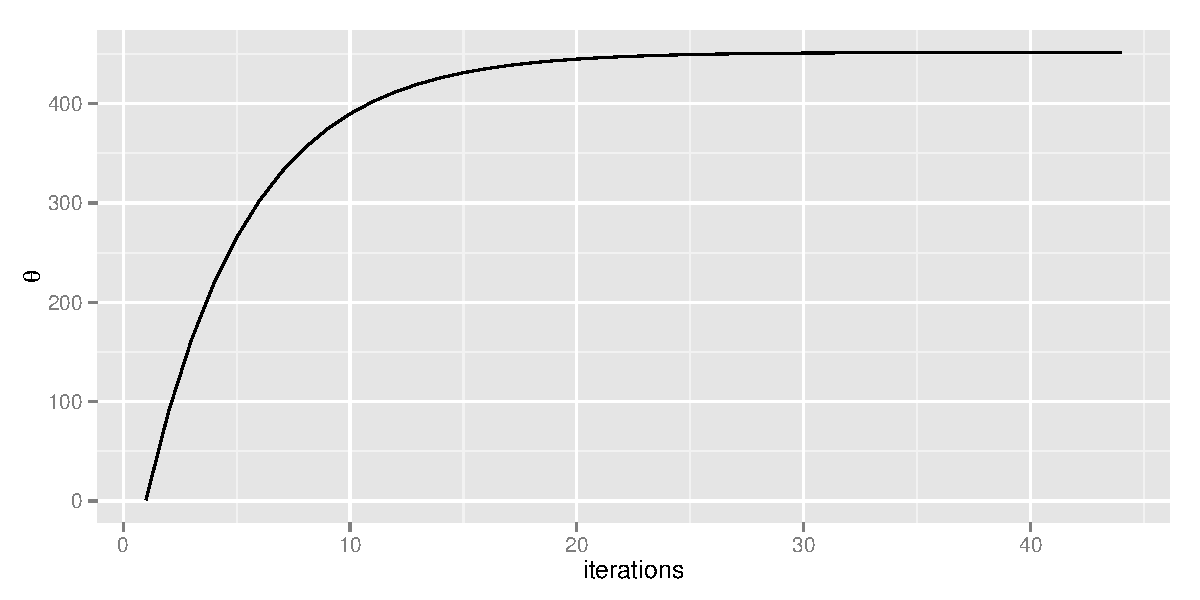
\includegraphics{aua257HW4-001}
\caption{Plot of $\theta$ vs. iterations}
\end{centering}
\end{figure}

Now we can choose a suitable starting value by calculating the MLE for the uncensored data ($<100$) assuming that follows a truncated exponential distribution. The starting value was found to be \textbf{244.9}. Running the algorithm for this starting value leads us to similar convergence as before.

For convergence criteria in this EM algorithm, at $k^{\text{th}}$ iterate, the absolute value of the difference of last two estimates i.e. $|\theta^{(k)}-\theta|$ is checked against some arbitrary pre-defined tolerance of $10^{-6}$. The algorithm is terminated when the difference becomes less than this tolerance.

%%%%%%%%%%%%%%%%%%%%%%%%%%%%%%%%%%%%%%%%%%%%%%%%%%%%%%%%%%%%%%%%%%%%%%%%%%%%%%%%%%%%%
\section*{Answer 3}
The final estimate of $\theta$ was obtained as \textbf{451.66}.

%%%%%%%%%%%%%%%%%%%%%%%%%%%%%%%%%%%%%%%%%%%%%%%%%%%%%%%%%%%%%%%%%%%%%%%%%%%%%%%%%%%%%
\section*{Answer 4}
Non-parametric bootstrap sampling was used to estimate the standard error estimate for $\hat{\theta}_{\text{EM}}$. The following steps describe the bootstrap approach:
\begin{enumerate}[label=(\alph*)]
\item Observed data $\utilde{Y}$ was resampled with replacement to obtain a Bootstrap sample $\utilde{Y}^*$.
\item For number of EM iterations defined as $50$ and starting value $451$, the EM algorithm was used to obtain MLE estimate $\hat{\theta}^*_{\text{EM}}$ for the bootstrap sample $\utilde{Y}^*$.

\item The above two steps were repeated $B$ times, where B is the Bootstrap sample size, to obtain $\hat{\theta}^{*(1)}_{\text{EM}}, \hat{\theta}^{*(2)}_{\text{EM}}, ...,  \hat{\theta}^{*(B)}_{\text{EM}}$. The sample standard deviation of $\hat{\theta}^{*(1)}_{\text{EM}}, \hat{\theta}^{*(2)}_{\text{EM}}, ...,  \hat{\theta}^{*(B)}_{\text{EM}}$ gives an estimate of standard error  for $\hat{\theta}_{\text{EM}}$. Note that, here B was chosen such that the absolute value of the difference of estimate of the standard error for $B$ and $(B-100)$ samples becomes less than an arbitrary pre-defined tolerance of $10^{-6}$.

\end{enumerate}

The estimate of the standard error obtained was \textbf{32.98}. The corresponding bootstrap sample size is \textbf{24208}.

The convergence of the standard error estimate with increasing number of bootstrap samples can be seen in the following plot.
\begin{figure}[H]
\begin{centering}
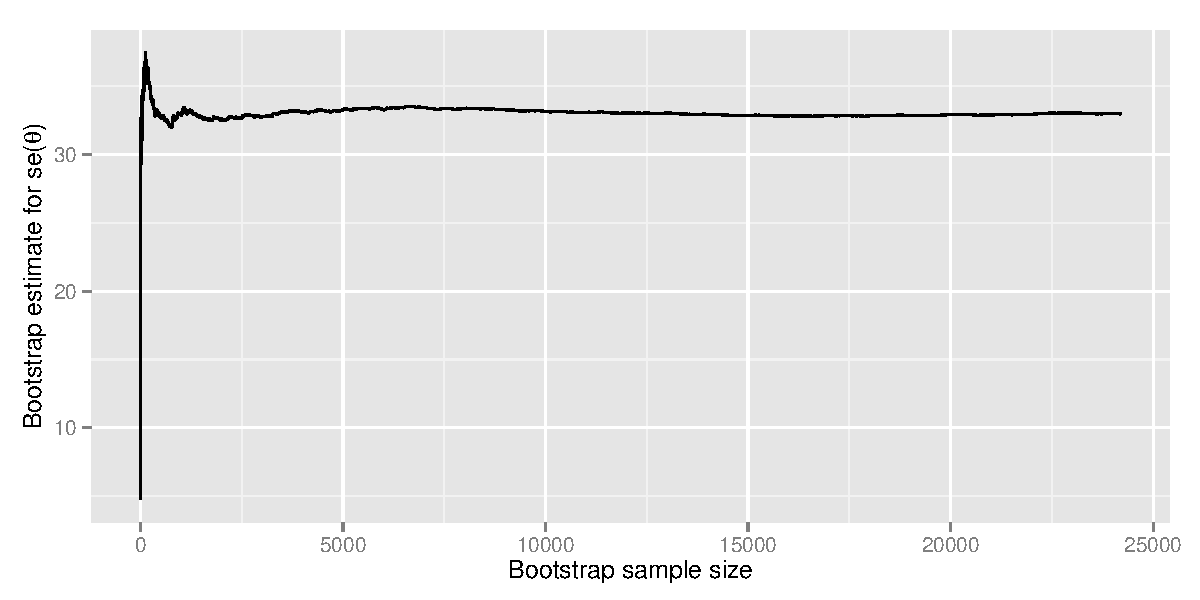
\includegraphics{aua257HW4-004}
\caption{Plot of se($\theta$) vs. Bootstrap sample size}
\end{centering}
\end{figure}

%%%%%%%%%%%%%%%%%%%%%%%%%%%%%%%%%%%%%%%%%%%%%%%%%%%%%%%%%%%%%%%%%%%%%%%%%%%%%%%%%%%%%
\section*{Answer 5}
The bootstrap 95\% t confidence interval for $\theta$ was obtained as (\textbf{378.28}, \textbf{506.38}).

%%%%%%%%%%%%%%%%%%%%%%%%%%%%%%%%%%%%%%%%%%%%%%%%%%%%%%%%%%%%%%%%%%%%%%%%%%%%%%%%%%%%%
\section*{Answer 6}

An alternative approach to obtain standard error estimates would be to compute the square root of inverse of the fisher information. This asymptotic approach is much easier to implement computationally atleast in this case since the fisher information $E\left(\dfrac{\partial^2 }{\partial \theta^2}(l_{\text{comp}}(\theta))\right)$ can be computed analytically. However for cases cases where this analytical calculation is not possible, the numerical approximation to the Fisher information might be too computationally expensive compared to Bootstrap approach.
\end{document}
